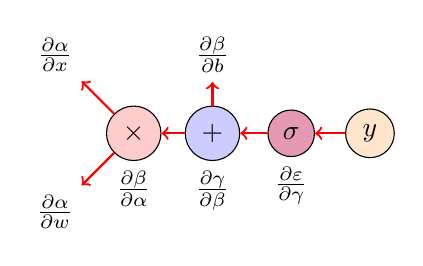
\begin{tikzpicture}[node distance=1cm]
    \node[draw, circle, fill=red!20, label=below:$\frac{\partial \beta}{\partial \alpha}$] (multiply) {$\times$};
    \node[draw, circle, fill=blue!20, right of=multiply, label=below:$\frac{\partial\gamma}{\partial\beta}$] (addition) {$+$};
    \node[draw, circle, fill=purple!40, right of=addition, label=below:$\frac{\partial \varepsilon}{\partial \gamma}$] (function) {$\sigma$};
    \node[draw, circle, fill=orange!20, right of=function] (output) {$y$};

    \draw[<-, thick, red] (multiply) -- (addition);
    \draw[<-, thick, red] (addition) -- (function);
    \draw[<-, thick, red] (function) -- (output);

    \node[left of=multiply, yshift=1cm,] (input1) {$\frac{\partial \alpha}{\partial x}$};
    \node[left of=multiply, yshift=-1cm,] (input2) {$\frac{\partial \alpha}{\partial w}$};
    \node[left of=addition, yshift=1cm, xshift=1cm,] (bias) {$\frac{\partial \beta}{\partial b}$};

    \draw[<-, thick, red] (input1) -- (multiply);
    \draw[<-, thick, red] (input2) -- (multiply);
    \draw[<-, thick, red] (bias) -- (addition);
\end{tikzpicture}